% \documentclass[fontsize=50pt, border=10pt, convert={outfile=\jobname.svg}]{standalone}
\documentclass[english, 12pt, border=10pt]{standalone}
\usepackage{tikz}
\usepackage{amsmath}
\usepackage{amssymb}
\usepackage{graphicx}
%%%%
% Provide the command \fpeval as a copy of the code-level \fp_eval:n.
%\usepackage{expl3}[2012-07-08]
\usepackage{expl3}
\ExplSyntaxOn
\cs_new_eq:NN \fpeval \fp_eval:n
\ExplSyntaxOff
%%%%
\usetikzlibrary{positioning}
\usetikzlibrary{decorations.pathreplacing,angles,quotes}
\usepackage{etoolbox}

\providecommand{\infig}{\includegraphics[width=50pt]{figs/chair1.jpg}}
\providecommand{\outfig}{\includegraphics[width=30pt]{figs/output_yes}}

\newtoggle{nolabel}
\toggletrue{nolabel}
\newtoggle{input}
\togglefalse{input}
% \definecolor{mygreen}{RGB}{0,180,0 }
% \definecolor{myblue}{RGB}{8,155,255}
% \definecolor{myred}{RGB}{250,0,0}
% net.add_color(name=r'inred', model='RGB', description="186,90,49")
% net.add_color(name=r'hidblue', model='RGB', description="49,160,180")
% net.add_color(name=r'outyellow', model='RGB', description="250,192,94")

% \definecolor{inc}{RGB}{186,90,49} % reddish
% \definecolor{hidc}{RGB}{49,160,180} % blue-ish
% \definecolor{outc}{RGB}{250,192,94} % yellow-ish

\definecolor{inc}{RGB}{134,166,165}
\definecolor{hidc}{RGB}{134,166,165}
\definecolor{outc}{RGB}{134,166,165}

\definecolor{weights}{RGB}{250,20,20}

\newcommand{\scale}{1.4}

\pgfdeclarelayer{bg}    % declare background layer
\pgfsetlayers{bg,main}  % set the order of the layers (main is the standard layer)

\begin{document}
%	\resizebox{12in}{!}{
		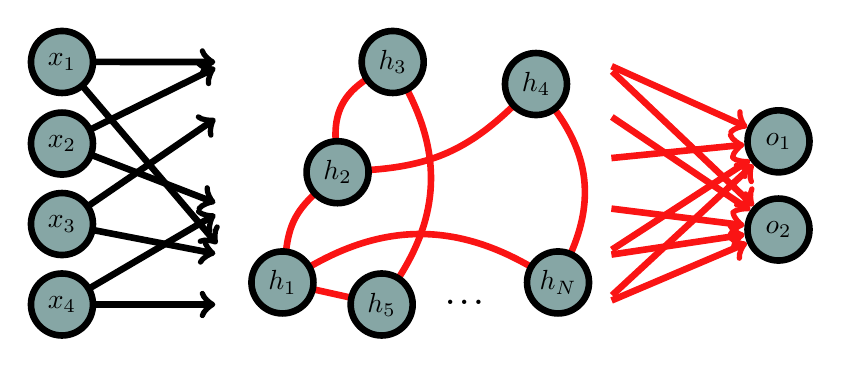
\begin{tikzpicture}[shorten >= 0pt, shorten <= -1pt, draw=black,line
		width=\fpeval{.5mm*\scale}, node distance=1cm, scale=\scale]
		%        \tikzstyle{every pin edge}=[<-,shorten <=1pt]
		\tikzstyle{neuron}=[circle,line
		width=\fpeval{.6mm*\scale},draw=black,fill=white,minimum
		size=\fpeval{16pt*\scale},inner sep=0pt]
		\tikzstyle{input neuron}=[neuron, fill=inc];
		\tikzstyle{hidden neuron}=[neuron, fill=hidc];
		\tikzstyle{output neuron}=[neuron, fill=outc];
		\tikzstyle{annot} = [text width=4em, text centered]
		\tikzstyle{ghost}=[opacity=0]
		\tikzstyle{trainweight}=[draw=weights, line width=\fpeval{.6mm*\scale}]
		\tikzstyle{weight}=[line width=\fpeval{.6mm*\scale}]
		\tikzstyle{rec_weight}=[line width=\fpeval{.6mm*\scale}, shorten >= -1pt, shorten <= -1pt]
		%        \tikzset{every path/.style={thick}}

		\node[input neuron](I1) at (-2,-.2) {$x_4$};
		\node[input neuron](I2) at (-2,0.53) {$x_3$};
		\node[input neuron](I3) at (-2,1.26) {$x_2$};
		\node[input neuron](I4) at (-2,2) {$x_1$};

		% \draw[decorate, decoration={brace, amplitude=15mm}, line width=1.25mm]   (I1.west) -- (I4.west);

		\newcommand{\gx}{-.5}
		\node[ghost](g1) at (\gx,-.2) {};
		\node[ghost](g2) at (\gx,0.24) {};
		\node[ghost](g3) at (\gx,0.68) {};
		\node[ghost](g4) at (\gx,1.12) {};
		\node[ghost](g5) at (\gx,1.56) {};
		\node[ghost](g6) at (\gx,2) {};


		\node[hidden neuron](N1) at (0,0) 		{$h_1$};
		\node[hidden neuron](N2) at (.5,1) 		{$h_2$};
		\node[hidden neuron](N3) at (1,2) 		{$h_3$};
		\node[hidden neuron](N4) at (.9,-.2)	{$h_5$};
		\node[annot] at (1.65, -.18)			{$\boldsymbol{\ldots}$};
		\node[hidden neuron](N5) at (2.5,0) 	{$h_N$};
		\node[hidden neuron](N6) at (2.3,1.8) 	{$h_4$};

		% \node[hidden neuron](N1) at (0,0)      {};
		% \node[hidden neuron](N2) at (.5,1)     {};
		% \node[hidden neuron](N3) at (1,2)      {};
		% \node[hidden neuron](N4) at (.8,-.2)   {};
		% \node[hidden neuron](N5) at (2.5,0)    {};
		% \node[hidden neuron](N6) at (2.3,1.8)  {};

		% \node[output neuron](O1) at (4.5,0.14) {\Huge $o_3$};
		% \node[output neuron](O2) at (4.5,0.88) {\Huge $o_2$};
		% \node[output neuron](O3) at (4.5,1.62) {\Huge $o_1$};
%		\node[neuron](O2) at (2.3,1.8) {\textcolor{red}{}};
%		\node[neuron](O3) at (2.3,1.8) {\textcolor{red}{}};

		% \node[output neuron](O1) at (4.5,0.14) {\Huge $o_3$};
		\node[output neuron](O1) at (4.5,0.48) {$o_2$};
		\node[output neuron](O2) at (4.5,1.28) {$o_1$};

		\newcommand{\gox}{2.9}
		\node[ghost](go1) at (\gox,-.2) {};
		\node[ghost](go2) at (\gox,0.24) {};
		\node[ghost](go3) at (\gox,0.68) {};
		\node[ghost](go4) at (\gox,1.12) {};
		\node[ghost](go5) at (\gox,1.56) {};
		\node[ghost](go6) at (\gox,2) {};

		\begin{pgfonlayer}{bg}
			% Recurrent Connections
			\path (N1) edge [trainweight, rec_weight, bend left = 20] (N2);
			\path (N3) edge [trainweight, rec_weight, bend right](N2);
			\path (N4) edge [trainweight, rec_weight, bend right = 30] (N3);
			\path (N1) edge [trainweight, rec_weight] (N4);
			\path (N1) edge [trainweight, rec_weight, bend left] (N5);
			\path (N5) edge [trainweight, rec_weight, bend right] (N6);
			\path (N6) edge [trainweight, rec_weight, bend left = 20] (N2);

			% Input Connections
			\path (I1) edge [weight, ->] (g3);
			\path (I3) edge [weight, ->] (g3);
			\path (I4) edge [weight, ->] (g2);
			\path (I2) edge [weight, ->] (g2);
			\path (I1) edge [weight, ->] (g1);
			\path (I4) edge [weight, ->] (g6);
			\path (I3) edge [weight, ->] (g6);
			\path (I2) edge [weight, ->] (g5);

			% Output Connections
			\path (go1) edge [trainweight, ->] (O1);
			\path (go2) edge [trainweight, ->] (O2);
			% \path (go3) edge [trainweight, ->] (O3);
			\path (go3) edge [trainweight, ->] (O1);
			\path (go4) edge [trainweight, ->] (O2);
			% \path (go5) edge [trainweight, ->] (O3);
			\path (go5) edge [trainweight, ->] (O1);
			\path (go6) edge [trainweight, ->] (O1);
			% \path (go6) edge [trainweight, ->] (O3);
			\path (go6) edge [trainweight, ->] (O2);
			\path (go1) edge [trainweight, ->] (O2);
			\path (go2) edge [trainweight, ->] (O1);
		\end{pgfonlayer}

		\end{tikzpicture}
%	}

\end{document}
